\section{Umsetzung des realen Clusters}
\label{sec:aufbauCluster}

Da die Plattform Hadoop"=Benchmark mithilfe von Docker auf einem physischen PC sehr einfach ein komplettes Hadoop"=Cluster ausführen kann, wurde die Plattform für diese Fallstudie als Basis genutzt.
Da Docker und Hadoop vor allem für den Einsatz in einer Linux"=Umgebung entwickelt wurden, werden für die Fallstudie zwei Computer genutzt, auf denen das Cluster wahlweise auf einem oder auf beiden Hosts ausgeführt werden kann.
Zudem wird auf einem Host eine VM mit Windows 10 ausgeführt, das zum Ausführen des .NET"=Frameworks bzw. \sS benötigt wird.
Beide zum Einsatz kommenden Hosts sind jeweils mit einem Intel Core i5"=4570 @ 3,2 GHz x 4, 16 GB Arbeitsspeicher sowie einer SSD ausgestattet, auf der Ubuntu 16.04 LTS installiert ist.
Die Verbindung von Windows zu Linux auf beiden Hosts wird mithilfe von SSH"=Verbindungen umgesetzt.

\begin{figure}
    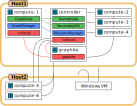
\includegraphics{./images/caseStudyHadoopSetup.pdf}
    \caption[In der Fallstudie verwendetes Cluster"=Setup]
    {In der Fallstudie verwendetes Cluster"=Setup.
        Grün: \ac{HDFS}, Blau: YARN, Rot: Graphite.}
    \label{fig:caseStudyHadoopSetup}
\end{figure}

\todo{Irgendwo erwähnen, wie Docker-Container aufeinander aufbauen}
Die beiden Abbildungen \autoref{fig:hadoopBenchmarkArchitecture} und \autoref{fig:caseStudyHadoopSetup} zeigen bereits den großen Hauptunterschied zwischen der Plattform und dem hier verwendeten Cluster"=Setup.
Da durch die Nutzung von virtuellen Maschinen ein zusätzlicher Ressourcenbedarf entsteht, wird im hier verwendeten Setup darauf verzichtet.
Durch die Ausführung der Docker"=Container des Hadoop"=Clusters direkt auf dem Host stehen dem Cluster mehr Ressourcen zur Verfügung.
Zudem wird es mithilfe von von \emph{Docker Swarm} so ermöglicht, das Hadoop"=Cluster auf beiden Hosts auszuführen.
Im konkreten Setup werden dabei Graphite, der Hadoop"=Controller sowie vier Hadoop"=Nodes auf dem Host1, sowie zwei weitere, optionale Nodes auf Host2 ausgeführt.
Weitere Anpassungen des verwendeten Setups bestehen \uA darin, dass der \ac{TLS} von Hadoop ebenfalls gestartet wird.
Zudem wurden einige Einstellungen von Hadoop so angepasst, dass defekte Nodes schneller erkannt werden.

Zum Ausführen der Windows"=VM auf Host2 wird VirtualBox 5.2 verwendet.
Zum Abrufen von Daten mithilfe der REST"=API von Hadoop über die SSH"=Verbindungen wird \emph{curl}\footnote{\url{https://curl.haxx.se/}} genutzt.
Zum Ausführen des Hadoop"=Clusters wird Docker in der Version 18.03 CE genutzt.

Um die in dieser Fallstudie benötigten Befehle einfach ausführen zu können, wurden zwei eigene Scripte erstellt, welche zum Teil auf den bestehenden Scripten der Plattform aufbauen.
Das Setup"=Script dient für folgende Zwecke:

\begin{itemize}
    \item Starten und Beenden des Clusters
    \item Starten und Beenden einzelner Hadoop"=Nodes
    \item Hinzufügen und Entfernen der Netzwerkverbindung des Docker"=Containers eines Hadoop"=Nodes
    \item Ausführen von eigenen Befehlen auf dem Docker"=Container des Hadoop"=Controllers
    \item Erstellen des Hadoop"=Docker"=Images
\end{itemize}

Das zweite erstellte Script dient ausschließlich zum Starten der Benchmarks.
Dazu werden die in der Plattform bereits enthaltenen Start"=Scripte aufgerufen, die für das konkrete Setup angepasst wurden.
